Commenting system is providing a function for user to communicate and see what they are feeling in for our product xxxxx.\par~

There are three parts of the function shown below.

\paragraph{Grading system}~

The grading system is providing two types of grading for student and professor.\par~


\includegraphics[scale=0.7]{Doc/Graphics/0star}


\includegraphics[scale=0.56]{Doc/Graphics/4star}

For the student, the grading system is the part for the user to express their feeling and show their satisfaction with our product or some of the interesting code in the forum.\par~

There are five stars for the grade. The user can click the button of the stars from left to right. After they clicked the button, the star buttons(s) is/are coloured. The user can click the most left that is the most unsatisfying star, while the most right that is showing the most satisfying.\par~

For the professor, the grading system is the part for the user to grade the masks of the program.\par~

The grade is shown in the digital number. The user can just type in the box of the grading system.

\paragraph{Reply system}~

Reply system is the part for the user to leave a message.\par~

User can leave any comment in comment box which is less than 1000 words.\par~

There are five buttons below.\par~

The commenting box that user can click to choose whether showing to the public, private or only for the administrator. the public option is for the user to share their ideas. The private option is for the user to make a remark for there own. The administrator option is for the user to make any suggestions to the system for further development of our product.\par~

Moreover, there are signed or unsigned options on the right hand side of the three options which mentioned. the user can choose to show name or not.

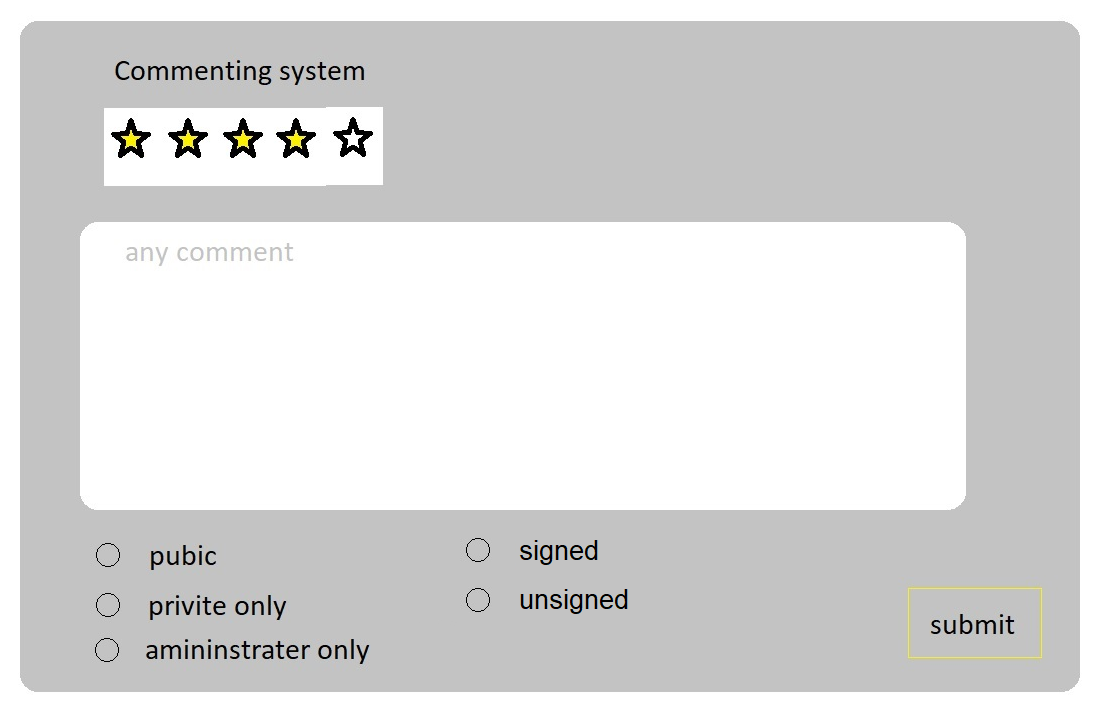
\includegraphics[scale=0.5]{Doc/Graphics/sdfg}

\paragraph{Deleting system}~

Deleting system is the part for the user to strike out useless message.\par~

The user can delete the comment by clicking the delete button which is on the right top corner.

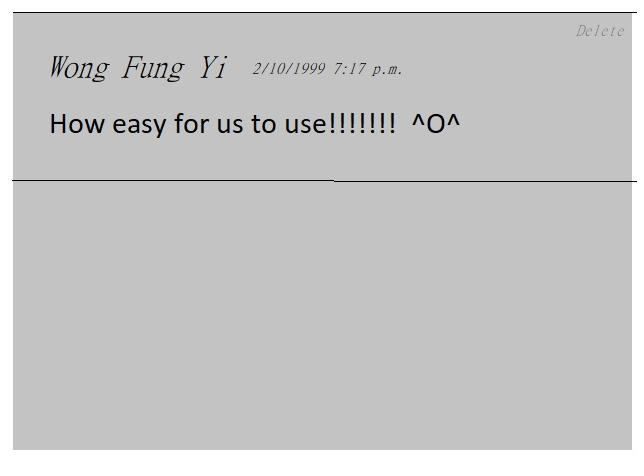
\includegraphics[scale=0.5]{Doc/Graphics/asdf}
